\chapter{Introduction}

Today, companies need to produce software faster than ever in order to remain competitive. To do so, they rely mainly on two different strategies: the integration of continuous deployment pipeline and the establishment of agile methodologies within the company. These strategies allow for software producers to increase the release rate while maintaining a high quality for the software that is shipped.

One of the keystones of the quality process is based on the adoption of automated software testing covering both functional and technical requirements which is providing a rapid feedback to the developers after each change to the system. In this work, we define testing as a technical investigation to assess the quality of a system under test (SUT) by executing the latter against a set of input values. Tests can further be classified through the scope they target into three categories: unit, integration and system tests. Unit testing cover the tests that are testing a unit, be it a class, a function or any other software component, in isolation to validate each unit individually. In integration testing, related modules are grouped together and tested as a group. Finally, system testing covers the test evaluating the system as a whole to evaluate its compliance to its requirements.

Because unit and integration tests target more restricted portions of the application, they offer better control to the tester who can isolate portions and tests the specific behavior of sub-parts of the system. On the other end, system tests and especially test interacting with the user interface, System User Interactive Tests (SUITs), tend to be more fragile, \ie\ they break following non-functional changes of the SUT.

In this work, we analyze the evolution of SUITs in order to shed light on the reason why these tests require costly maintenance. Then, we propose some solutions as how to create more robust test suites, \ie, test suites that are less likely to break following non-functional evolution of the system under while exhibiting a more stable behavior.


\section{Testing through the User Interfaces}

User Interfaces are designed to provide a way for the user to interact with an application. Unfortunately, as interfaces become more user-friendly, the underlying technology becomes more complex \cite{Myers1994}. Indeed, as depicted by \citep{Myers1995}, user interfaces require the system to  interact with complex graphical components, to provide multiple ways to provide the same command, to manage multiple asynchronous input devices through the use of asynchronous event loops, to provide an interactive computer programming environment (\eg\ read–evaluate–print loop), etc. Thus, to ease development, different architectural designs are proposed in the literature to decouple the code responsible for the user interaction to the rest of the system such as the Entity-Component-System model \cite{Raffaillac2018}.

Nevertheless, while these architectural solutions, providing better isolation, offer advantages when testing individual components, in the case of system testing, the challenges remain open. Indeed, as the complexity of user interfaces and their associated code continues to grow, testing through the user interface for functional correctness remains challenging, but vital to help ensure the safety, robustness and usability of the SUT. The question is of utmost importance since developers report that prototyping and developing the behavior of a system is harder than prototyping and developing the appearance of the application \cite{Myers2008}.

Today, Graphical User Interface (GUI) are becoming ubiquitous as a mean for users to interact with a software \cite{Myers1992, Myers1995, Brooks2009}. A GUI-based application can be defined as a software for which the GUI is the main mode of interaction to the detriment of other types of user interfaces. Thus, a lot of effort have been geared towards GUI automation explaining the abundance of SUITs frameworks targeting specifically GUI-based applications.

%An event-flow model of GUI-based applications for testing

In the remainder of this section, we discuss current techniques used to test application through their interfaces. Different approaches are order in term of creation effort.

\subsection{Random GUI Testing}
\label{sec:introduction-random-gui-testing}

\subsection{Capture \& Replay}
\label{sec:introduction-capture-and-replay}

As its name suggests, Capture \& Replay works in two phases: a capture phase and a replay phase. During the capture phase, the tester manually interacts with the application, thereby generating events on the SUT. The tool records the interactions and a part of the SUT response state as specified by the tester. Then, during the replay phase, the recorded test cases can be replayed on subsequent versions of the SUT and the captured state of the application are used as test oracles.

\subsection{Test Scripting}
\label{sec:introduction-test-scripting}

Keyword-Driven testing (KDT) is a software testing technique that aims at separating test design from the technical implementation of the tests, thus, limiting exposure to unnecessary details and avoiding duplication. KDT advocates that this separation of concerns allows tests to be written easier, to create more maintainable tests and enables experts from different fields and backgrounds to work together, at different levels of abstraction, for the creation of the tests.

To do so, KDT\cite{Tang2008} aims at separating test design from technical implementation. Its goal is to limit the exposure to unnecessary details and avoiding duplication. KDT advocates that this separation of concerns allows tests to be written easier, to create more maintainable tests and enables experts from different fields and backgrounds, work together at different levels of abstraction. 

Listing~\ref{lst:robot} shows an example of a KDT test. This test, named ``Valid Login'' (line 5, adopted from the official documentation of Robot Framework), is responsible for validating the correct behaviour of the login form in an imaginary SUT. Lines 6--8 present the ``steps'' of the tests and, in KDT parlance, they are calls to \emph{keywords}. In turn, these keywords are defined in the respective definition blocks between lines 10 and 28. Each keyword is itself decomposed in a series of steps. Keywords can have \emph{arguments}. For instance, keyword ``Open browser'' (line 12) takes two arguments, ``\$\{LOGIN URL\}'' and ``\$\{BROWSER\}''. The use of arguments to call keywords allows to further extend the reuse of keywords.

As can be seen from the figure, most part of this fully automated test is written in plain English. This enables the unobstructed collaboration in the creation of the tests between different experts. For instance, a business analyst can write the high-level part of the test (lines 4--8) and an automation expert can implement the remaining part of the test (lines 10-35), adding the technical details to automate the steps.

\begin{lstlisting}[caption={Example of Robot Framework test}, label={lst:robot}]
    <@\textcolor{block}{*** Settings ***}@>
    Test Teardown     Close All Browsers
    Library           Selenium2Library    run_on_failure=Capture Page Screenshot
    
    <@\textcolor{block}{*** Test Cases ***}@>
    <@\textcolor{keyword}{A user logs in with his username and password}@>
        Given browser is opened to login page
        When user "demo" logs in with password "mode"
        Then welcome page should be open
    
    <@\textcolor{block}{*** Keywords ***}@>
    <@\textcolor{keyword}{Browser is opened to login page}@>
        Open browser to login page
    
    <@\textcolor{keyword}{User "}@><@\textcolor{variable}{\$\{username\}}@><@\textcolor{keyword}{" logs in with password "}@><@\textcolor{variable}{\$\{password\}}@><@\textcolor{keyword}{"}@>
        Input username    <@\textcolor{variable}{\$\{username\}}@>
        Input password    <@\textcolor{variable}{\$\{password\}}@>
        Submit credentials
    
    <@\textcolor{keyword}{Open Browser To Login Page}@>
        Open Browser    <@\textcolor{variable}{\$\{LOGIN URL\}}@>    <@\textcolor{variable}{\$\{BROWSER\}}@>
        Maximize Browser Window
        Set Selenium Speed    0
        Login Page Should Be Open        
    
    <@\textcolor{keyword}{Go To Login Page}@>
        Go To    <@\textcolor{variable}{\$\{LOGIN URL\}}@>
        Login Page Should Be Open
    
    <@\textcolor{keyword}{Input Username}@>
        [Arguments]    <@\textcolor{variable}{\$\{username\}}@>
        Input Text    username_id    <@\textcolor{variable}{\$\{username\}}@>
    
    <@\textcolor{keyword}{Input Password}@>
        [Arguments]    <@\textcolor{variable}{\$\{password\}}@>
        Input Text    password_id    <@\textcolor{variable}{\$\{password\}}@>
    
    <@\textcolor{keyword}{Submit Credentials}@>
        Click Button    validate_id
        
    <@\textcolor{keyword}{Welcome Page Should Be Open}@>
        Title Should Be    Welcome Page
        
    <@\textcolor{keyword}{Login Page Should Be Open}@>
        Title Should Be    Login Page
    
    <@\textcolor{block}{*** Variables ***}@>
        <@\textcolor{variable}{\$\{SERVER\}}@>           localhost:7272
        <@\textcolor{variable}{\$\{BROWSER\}}@>          Chrome        
        <@\textcolor{variable}{\$\{LOGIN URL\}}@>        http://<@\textcolor{variable}{\$\{SERVER\}}@>
\end{lstlisting}

KDT tests can be represented using a tree structure. Figure~\ref{fig:robotframework_tree} shows this structure for the test of Listing~\ref{lst:robot}. The root of the tree (purple rectangle) is the \emph{Test Case} that is executed by calling all the keywords contained. The intermediary nodes (white rectangles) are called \emph{User Keywords} since they are created by the tester. Finally, the leaf nodes (green rectangles) are \emph{Library Keywords}. \emph{Library Keywords} are implemented by the system or an external library and responsible for either controlling the control flow of the tests or interacting with the SUT.

\begin{figure}
\centering
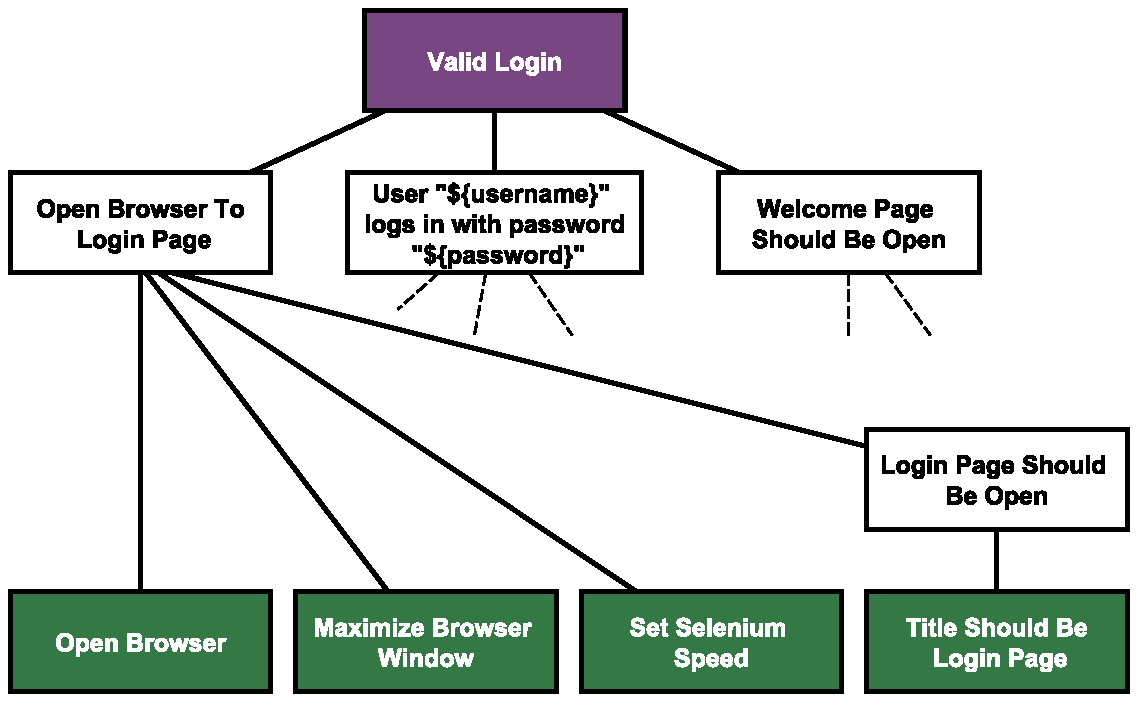
\includegraphics[width=\columnwidth]{figures/evolution/robotframework_tree.pdf}
\caption{Tree representation of the ``Valid Login'' KDT test.}
\label{fig:robotframework_tree}
\end{figure}

We group keywords into seven categories based on their functionality and present them in Table \ref{keywords_categories}. We define a \emph{SYNC}
keyword category for keywords dealing with the synchronization between tests and SUT; e.g., a keyword that waits 10 seconds for a GUI element of the SUT to become available. In the rest of the paper we use the term keyword to refer to \emph{User Keywords} unless stated otherwise.

One the tools used for the application of KDT is Robot Framework \cite{RobotFramework2020}. Robot Framework is a popular framework used world-wide by major companies, including Nokia, KONE, ABB. This is also the tool adopted by our industrial partner and, thus, used in this work. Robot Framework is an open source tool originally developed by Nokia Networks and is mainly used for acceptance testing. The ``Valid Login'' KDT test of Listing~\ref{lst:robot} was written using this framework.

One of the main advantages of Robot Framework is its high modularity.  Indeed, Robot Framework is platform-agnostic and thanks to its driver plugin architecture, the core framework does not require any knowledge of the SUT. For instance, in Listing~\ref{lst:robot}, lines 1--2 show that the script is using the external library for Selenium to interact with the SUT. Another advantage of the framework lies in its simple syntax, which makes it easily accessible to testers, regardless of their background.

\begin{table}
\caption{Keyword categories}
\label{keywords_categories}
\centering
\begin{tabular}{>{\raggedright}m{0.9in}>{\raggedright}m{4in}}
\toprule
\textbf{\scriptsize{Label}} & \textbf{\scriptsize{Explanation}}\tabularnewline
\toprule

\scriptsize{\textit{ACTION}} & \scriptsize{Keyword performing an action on the
SUT capable of modifying its state.} \tabularnewline

\scriptsize{\textit{ASSERTION}} & \scriptsize{Keyword verifying that a predicate
is true at a specific point of test execution} \tabularnewline

\scriptsize{CONTROLFOW} & \scriptsize{Keyword allowing to modify the
                                   control flow of the test execution.} \tabularnewline

\scriptsize{GETTER} & \scriptsize{Keyword allowing to extract an element from
the SUT.} \tabularnewline

\scriptsize{LOGGING} & \scriptsize{Keyword dumping logs during execution.}
\tabularnewline

\scriptsize{SYNC} & \scriptsize{Keyword relating to the
                                  synchronization between the SUT and the tests.} \tabularnewline

\scriptsize{\textit{USER}} & \scriptsize{Keyword created by a user.}
\tabularnewline

\bottomrule
\end{tabular}
\end{table}

\subsection{Model-Based Testing}

\section{Challenges of System User Interactive Tests}

\subsection{The Added Value of System User Interactive Tests}

\subsection{The Fragility Problem}

\section{Overview of the Contribution and Organization of the Dissertation}
\subsection{Contributions}
\subsection{Organization of the Dissertation}